% Tento soubor je GENEROVANY - needitujte ho.
% Zdroj: strom_obojzivelnici_long.drawio
% Generuje R/05_metodiky/51_metodika_diagramy.R z predlohy v Diagrams/.
\documentclass[border=2pt]{standalone}
\usepackage[utf8]{inputenc}
\usepackage[T1]{fontenc}
\usepackage[scaled]{helvet}
\renewcommand{\familydefault}{\sfdefault}
\usepackage{tikz}
\usetikzlibrary{arrows.meta}
% draw.io slova nedeli - zakaz deleni drzi zlomy radku na stejnych mistech
\hyphenpenalty=10000
\exhyphenpenalty=10000
\hbadness=10000
\definecolor{dio006C4E}{HTML}{006C4E}
\definecolor{dioFFFFFF}{HTML}{FFFFFF}
\definecolor{dioCD011A}{HTML}{CD011A}
\definecolor{dio000000}{HTML}{000000}
\definecolor{dioF59B23}{HTML}{F59B23}
\definecolor{dio94F204}{HTML}{94F204}
\definecolor{dioEFEEED}{HTML}{EFEEED}
\begin{document}
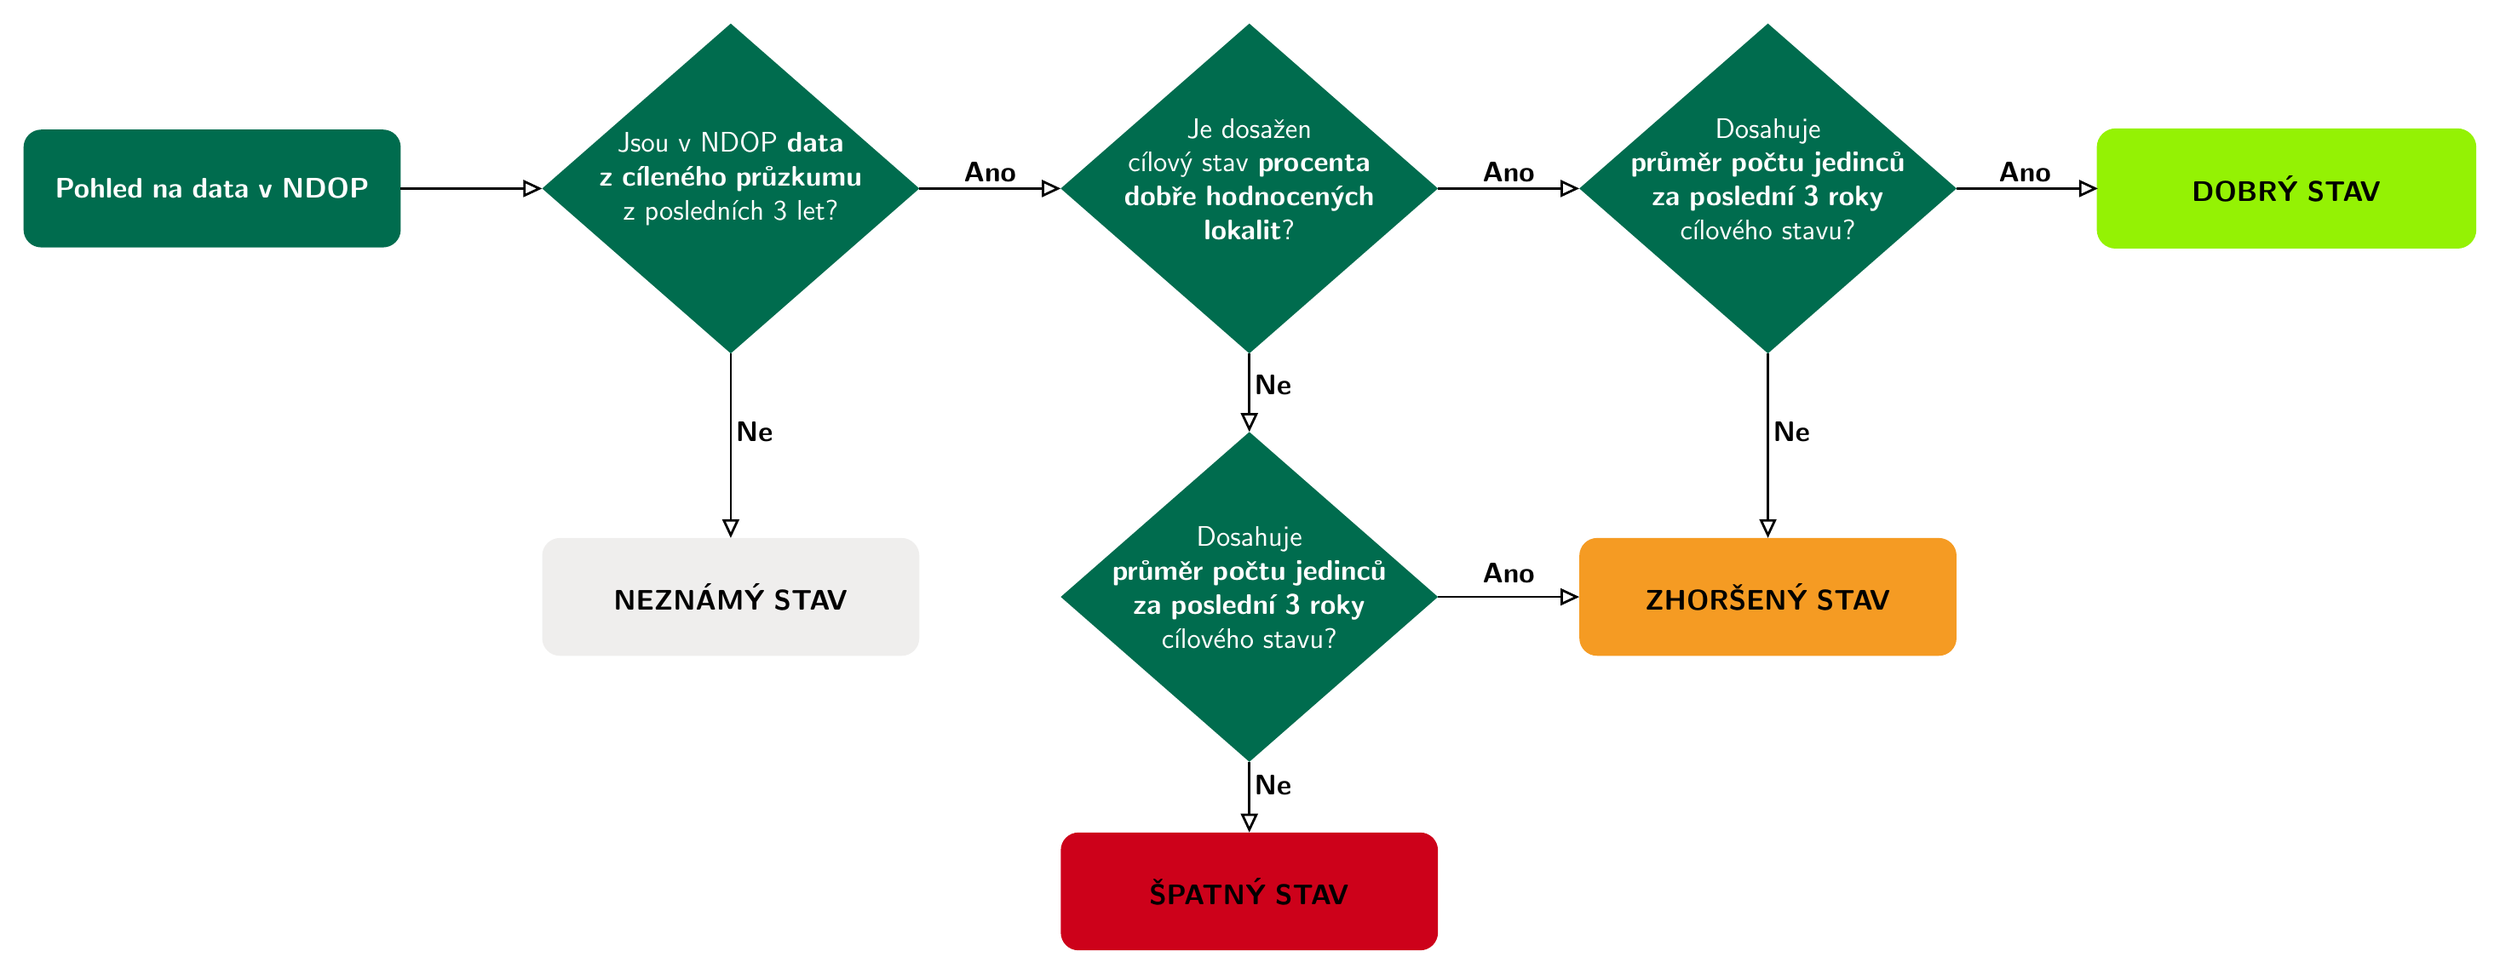
\begin{tikzpicture}[x=1.0000pt, y=-1.0000pt, line cap=butt, line join=miter]
  \path[fill=dio006C4E, draw=none, line width=1.00pt, rounded corners=7.50pt] (27.00,241.67) rectangle (187.00,291.67);
  \node[align=center, inner sep=0pt, outer sep=0pt, text=dioFFFFFF, font=\fontsize{12.00}{14.40}\selectfont, text width=156.00pt] at (107.00,266.67) {\textbf{Pohled na data v NDOP}};
  \path[fill=dio006C4E, draw=none, line width=1.00pt] (547.00,196.67) -- (627.00,266.67) -- (547.00,336.67) -- (467.00,266.67) -- cycle;
  \node[align=center, inner sep=0pt, outer sep=0pt, text=dioFFFFFF, font=\fontsize{12.00}{14.40}\selectfont, text width=148.00pt] at (547.00,262.67) {Je dosažen\\cílový stav \textbf{procenta}\\\textbf{dobře hodnocených}\\\textbf{lokalit}?};
  \path[fill=dio006C4E, draw=none, line width=1.00pt] (547.00,370.00) -- (627.00,440.00) -- (547.00,510.00) -- (467.00,440.00) -- cycle;
  \node[align=center, inner sep=0pt, outer sep=0pt, text=dioFFFFFF, font=\fontsize{12.00}{14.40}\selectfont, text width=148.00pt] at (547.00,436.00) {Dosahuje\\\textbf{průměr počtu jedinců}\\\textbf{za poslední 3 roky}\\cílového stavu?};
  \path[fill=dio006C4E, draw=none, line width=1.00pt] (767.00,196.67) -- (847.00,266.67) -- (767.00,336.67) -- (687.00,266.67) -- cycle;
  \node[align=center, inner sep=0pt, outer sep=0pt, text=dioFFFFFF, font=\fontsize{12.00}{14.40}\selectfont, text width=148.00pt] at (767.00,262.67) {Dosahuje\\\textbf{průměr počtu jedinců}\\\textbf{za poslední 3 roky}\\cílového stavu?};
  \path[fill=dioCD011A, draw=none, line width=1.00pt, rounded corners=7.50pt] (467.00,540.00) rectangle (627.00,590.00);
  \node[align=center, inner sep=0pt, outer sep=0pt, text=dio000000, font=\fontsize{12.00}{14.40}\selectfont, text width=156.00pt] at (547.00,565.00) {\textbf{ŠPATNÝ STAV}};
  \path[fill=dioF59B23, draw=none, line width=1.00pt, rounded corners=7.50pt] (687.00,415.00) rectangle (847.00,465.00);
  \node[align=center, inner sep=0pt, outer sep=0pt, text=dio000000, font=\fontsize{12.00}{14.40}\selectfont, text width=156.00pt] at (767.00,440.00) {\textbf{ZHORŠENÝ STAV}};
  \path[fill=dio94F204, draw=dio94F204, line width=1.00pt, rounded corners=7.50pt] (907.00,241.67) rectangle (1067.00,291.67);
  \node[align=center, inner sep=0pt, outer sep=0pt, text=dio000000, font=\fontsize{12.00}{14.40}\selectfont, text width=156.00pt] at (987.00,266.67) {\textbf{DOBRÝ STAV}};
  \path[fill=dio006C4E, draw=none, line width=1.00pt] (327.00,196.67) -- (407.00,266.67) -- (327.00,336.67) -- (247.00,266.67) -- cycle;
  \node[align=center, inner sep=0pt, outer sep=0pt, text=dioFFFFFF, font=\fontsize{12.00}{14.40}\selectfont, text width=148.00pt] at (327.00,262.67) {Jsou v NDOP \textbf{data}\\\textbf{z cíleného průzkumu}\\z posledních 3 let?};
  \path[fill=dioEFEEED, draw=none, line width=1.00pt, rounded corners=7.50pt] (247.00,415.00) rectangle (407.00,465.00);
  \node[align=center, inner sep=0pt, outer sep=0pt, text=dio000000, font=\fontsize{12.00}{14.40}\selectfont, text width=156.00pt] at (327.00,440.00) {\textbf{NEZNÁMÝ STAV}};
  \draw[draw=dio000000, line width=1.00pt, -{Triangle[length=8.00pt, width=7.20pt, color=dio000000, fill=white, line width=1.00pt]}] (627.00,266.67) -- (687.00,266.67);
  \node[align=center, inner sep=0pt, outer sep=0pt, text=dio000000, font=\fontsize{12.00}{14.40}\selectfont] at (657.00,259.67) {\textbf{Ano}};
  \draw[draw=dio000000, line width=1.00pt, -{Triangle[length=8.00pt, width=7.20pt, color=dio000000, fill=white, line width=1.00pt]}] (547.00,336.67) -- (547.00,370.00);
  \node[align=center, inner sep=0pt, outer sep=0pt, text=dio000000, font=\fontsize{12.00}{14.40}\selectfont] at (557.00,350.00) {\textbf{Ne}};
  \draw[draw=dio000000, line width=1.00pt, -{Triangle[length=8.00pt, width=7.20pt, color=dio000000, fill=white, line width=1.00pt]}] (547.00,510.00) -- (547.00,540.00);
  \node[align=center, inner sep=0pt, outer sep=0pt, text=dio000000, font=\fontsize{12.00}{14.40}\selectfont] at (557.00,520.00) {\textbf{Ne}};
  \draw[draw=dio000000, line width=1.00pt, -{Triangle[length=8.00pt, width=7.20pt, color=dio000000, fill=white, line width=1.00pt]}] (767.00,336.67) -- (767.00,415.00);
  \node[align=center, inner sep=0pt, outer sep=0pt, text=dio000000, font=\fontsize{12.00}{14.40}\selectfont] at (777.00,370.00) {\textbf{Ne}};
  \draw[draw=dio000000, line width=1.00pt, -{Triangle[length=8.00pt, width=7.20pt, color=dio000000, fill=white, line width=1.00pt]}] (847.00,266.67) -- (907.00,266.67);
  \node[align=center, inner sep=0pt, outer sep=0pt, text=dio000000, font=\fontsize{12.00}{14.40}\selectfont] at (876.00,259.67) {\textbf{Ano}};
  \draw[draw=dio000000, line width=1.00pt, -{Triangle[length=8.00pt, width=7.20pt, color=dio000000, fill=white, line width=1.00pt]}] (627.00,440.00) -- (687.00,440.00);
  \node[align=center, inner sep=0pt, outer sep=0pt, text=dio000000, font=\fontsize{12.00}{14.40}\selectfont] at (657.00,430.00) {\textbf{Ano}};
  \draw[draw=dio000000, line width=1.00pt, -{Triangle[length=8.00pt, width=7.20pt, color=dio000000, fill=white, line width=1.00pt]}] (407.00,266.67) -- (467.00,266.67);
  \node[align=center, inner sep=0pt, outer sep=0pt, text=dio000000, font=\fontsize{12.00}{14.40}\selectfont] at (437.00,259.67) {\textbf{Ano}};
  \draw[draw=dio000000, line width=1.00pt, -{Triangle[length=8.00pt, width=7.20pt, color=dio000000, fill=white, line width=1.00pt]}] (187.00,266.67) -- (247.00,266.67);
  \draw[draw=dio000000, line width=1.00pt, -{Triangle[length=8.00pt, width=7.20pt, color=dio000000, fill=white, line width=1.00pt]}] (327.00,336.67) -- (327.00,415.00);
  \node[align=center, inner sep=0pt, outer sep=0pt, text=dio000000, font=\fontsize{12.00}{14.40}\selectfont] at (337.00,370.00) {\textbf{Ne}};
\end{tikzpicture}
\end{document}
